\documentclass[12pt]{beamer}
\usepackage[utf8]{inputenc}
\usepackage{lmodern}
\usepackage[spanish]{babel}
\usetheme{metropolis}
\usepackage{graphicx}

\begin{document}
	\author{Citruxs}
	\title{Git  (No confundir con GitHub)}
	%\subtitle{}
	%\logo{}
	%\institute{}
	%\date{}
	%\subject{}
	%\setbeamercovered{transparent}
	%\setbeamertemplate{navigation symbols}{}
	\begin{frame}[plain]
		\maketitle
	\end{frame}
	
	\begin{frame}
		\frametitle{¿Qué es Git?}
		Git es un software de control de versiones, pensando en la eficiencia, la confiabilidad y compatibilidad del mantenimiento de versiones de aplicaciones cuando están tienen un gran número de archivos.
		
		Algunos beneficios de su uso son:
		\begin{itemize}
			\item Desarrollo distribuido
			\item Historial de cambios
			\item Rastreo de errores
		\end{itemize}
	\end{frame}
	
	\begin{frame}
		\frametitle{Instalación de Git}
		La instalación de Git dependerá del sistema operativo en el que te encuentres
		\begin{itemize}
			\item Windows: \url{https://git-scm.com/download/win}
			\item MacOS: Usa Homebrew: brew install git
			\item Linux: sudo apt-get install git (Ubuntu/Debian), sudo dnf install git (CentOS/RHEL)
		\end{itemize}
		Para verificar la versión de git con la que cuentas solo hace falta escribir sobre la terminal 'git --version'
	\end{frame}
	
	\begin{frame}
		\frametitle{Configuracion de Git}
		Una vez que Git está instalado en nuestro sistema solo hace falta configurar el nombre y correo electrónico con el que los commits serán asociados.
		
		\begin{itemize}
			\item git config --global user.name ``Robocop Pérez"
			\item git config --global user.email ``robocop.perez@example.com"
		\end{itemize}
	\end{frame}
	
	\begin{frame}
		\frametitle{Creación y uso de un repositorio}
		\framesubtitle{Creación del repositorio}
		Una manera sencilla de iniciar un repositorio es ubicarnos sobre la carpeta donde estará alojado nuestro repositorio, abrir la terminal y escribir:
		\begin{itemize}
			\item git init
		\end{itemize}
		Podemos verificar que el repositorio esta hecho con:
		
		\begin{itemize}
			\item git status
		\end{itemize}
		
		Una buena practica para el uso de repositorios en Git es agregar un archivo readme, pues en este se suele agregar un resumen sobre el repositorio en el que se trabaja, así como instrucciones en general, el formato de este archivo debe de ser .md
	\end{frame}
	
	\begin{frame}
		\framesubtitle{Estatus de archivos}
		Git tiene tres etiquetas distintas para identificar el estatus en el que se encuentran los archivos dentro del repositorio
		
		\begin{itemize}
			\item modificado: Son los archivos que hemos modificado desde la ultima versión ``oficial" que tenemos en el repositorio.
			\item preparado (stagged) : Son los archivos a los que ya hemos hecho modificaciones pero con la diferencia de que está preparado para reportar los cambios.
			\item confirmado (committed): Son los archivos los cuales ya tienen los cambios reportados.
		\end{itemize}
		
		Veamos un ejemplo creando nuestro archivo README.md en un repositorio de prueba
	\end{frame}
	
	\begin{frame}
		\framesubtitle{Ejemplo con README.md}
		Una vez que hemos creado el archivo README.md o hecho algún cambio sobre el repositorio podemos verificar los cambios
		
		\begin{figure}[h]
			\centering
			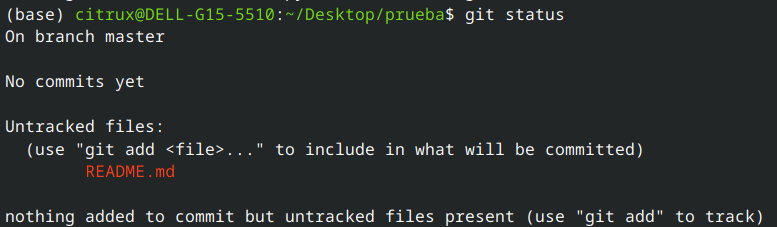
\includegraphics[width=0.75\textwidth]{Imagenes/git_status.png}
		\end{figure}
		
		Así vemos que en la sección de untracked files nos indica que el archivo README.md tiene cambios pero no están siendo reportados en el repositorio.
		
	\end{frame}
	
	\begin{frame}
		\framesubtitle{git add}
		 Reportaremos los cambios del archivo README.md, para esto usamos la siguiente instrucción
		
		\begin{itemize}
			\item git add README.md
			\item Una alternativa es usar 'git add .', con esta instrucción le indicamos a git que agregue todos los cambios que hemos hecho en todo el repositorio (No es recomendable usarlo si hemos echo diferentes tipo de cambios) 
		\end{itemize}
		
		\begin{figure}[h]
			\centering
			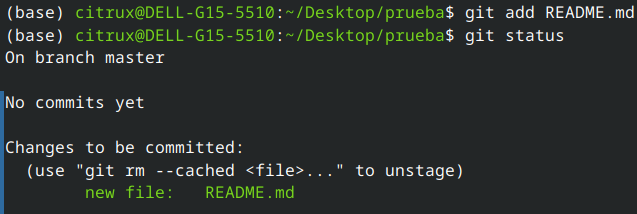
\includegraphics[width=0.75\textwidth]{Imagenes/git_add.png}
		\end{figure}
	\end{frame}
	
	\begin{frame}
		\framesubtitle{git commit}
		Una vez que los cambios están listos para ser reportados, comentamos brevemente los cambios que hemos hecho, para esto usamos:
		
		\begin{itemize}
			\item git commit -m ``Inserte un comentario ingenioso"
		\end{itemize}
		
		\begin{figure}[h]
			\centering
			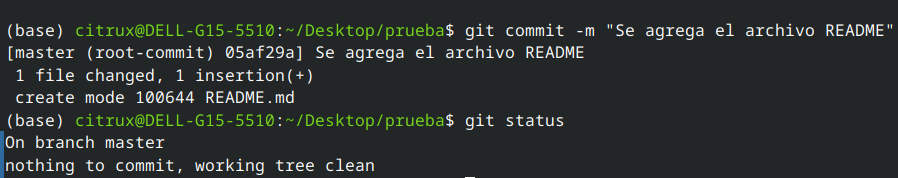
\includegraphics[width=0.9\textwidth]{Imagenes/git_commit.png}
		\end{figure}
	\end{frame}
	
	\begin{frame}
		Y listo, nuestros cambios han sido correctamente reportados y podemos visualizar el historial de cambios con:
		\begin{itemize}
			\item git log
		\end{itemize}
		
		\begin{figure}[h]
			\centering
			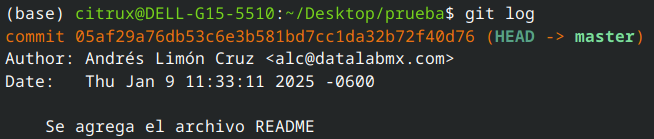
\includegraphics[width=0.9\textwidth]{Imagenes/git_log.png}
		\end{figure}
	\end{frame}
	
	\begin{frame}
		\frametitle{Extras}
		-¿Que pasa si eliminé por equivocación algún archivo de mi repositorio?
		
		Afortunadamente git al ayudarnos a rastrear los cambios dentro de nuestro repositorio nota la eliminación de archivos, y podemos recuperarlos fácilmente con:
		\begin{itemize}
			\item git restore ``Nombre del archivo"
			\item git restore . (Esto recupera todos los archivos borrados desde el ultimo cambio registrado en el repositorio)
		\end{itemize}
	\end{frame}
	
	\begin{frame}
		-Tengo archivos que no me gustaría incluir para reportar mis cambios, ¿Cómo hago que git los ignore?
		
		Para esto ocupamos un tipo de archivo especial para que git sepa que archivos no debe incluir, este tipo de archivo debe tener un nombre especial ``.gitignore`` y en el agregamos el nombre de los archivos que no incluiremos o la terminación de archivos que ignoraremos
		
		\begin{figure}[h]
			\centering
			\includegraphics[width=0.9\textwidth]{Imagenes/git_ignore.png}
		\end{figure}
		
	\end{frame}
	
	\begin{frame}
		-Hice cambios en un archivo, pero quiero revertirlo a su estado original, ¿Cómo lo hago?
		
		Si este es tu caso, git tiene una instrucción especial para revertir los cambios en los archivos, esta instrucción es: ``git checkout -- archivo"
		
		-Añadí un archivo al área de preparación (stagged), ¿Cómo lo regreso al área de modificados?
		
		En este caso se usa: ``git reset archivo.txt"

	\end{frame}

	\begin{frame}
		-¿Cómo deshago algún commit?\\
		Si tenemos algún commit que no queremos mantener lo podemos realizar de 2 maneras:\\
		Perdiendo todos los cambios que se realizaron después de ese commit:\\
		``git reset --hard HEAD\textasciitilde n", con n indicamos que commit borraremos\\
		Borrando solo ese commit y manteniendo los posteriores:\\
		``git reset --soft HEAD\textasciitilde n"
	\end{frame}
	
	\begin{frame}
			\begin{figure}[h]
			\centering
			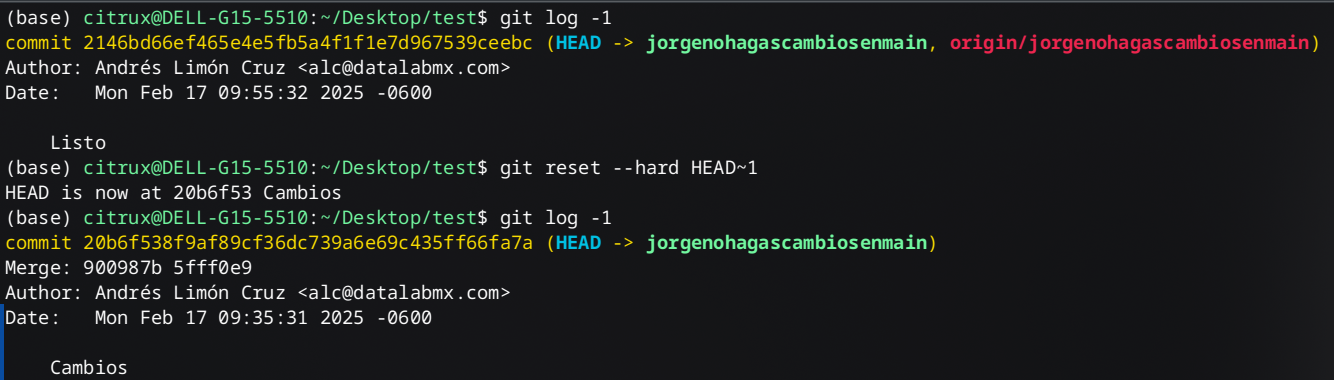
\includegraphics[width=0.9\textwidth]{Imagenes/git_reset_commit.png}
		\end{figure}
	\end{frame}
	
	
	\begin{frame}
		\frametitle{Último extra: Ramas (Branchs)}
		Una buena practica al momento de trabajar con git es el uso de ramas, podemos pensar en un repositorio git como un árbol, donde el tronco representa la rama maestra pues es la principal, ya que contiene la versión que sale a producción.
		
		Si realizamos cambios de los cuales no estamos seguros sobre el efecto que pueden tener en la versión de producción lo mejor es usar una rama donde guardaremos nuestros cambios y en su momento uniremos de nuevo con la versión de producción.
	\end{frame}
	
	\begin{frame}
		\framesubtitle{Ramas: Continuación}
		Podemos verificar las ramas que existen en nuestro repositorio con: ``git branch"
		\begin{figure}[h]
			\centering
			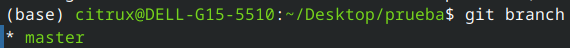
\includegraphics[width=0.9\textwidth]{Imagenes/git_branch.png}
		\end{figure}
		
		Podemos crear una nueva branch y verificar en que rama estamos
		
		\begin{figure}[h]
			\centering
			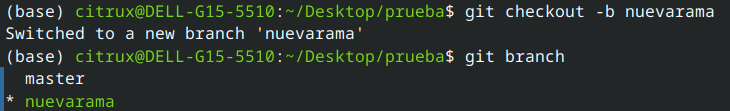
\includegraphics[width=0.9\textwidth]{Imagenes/git_nuevarama.png}
		\end{figure}
		
	\end{frame}
	
	\begin{frame}
		Podemos volver a la rama master con: ``git switch nombre\_de\_la\_rama" o con ``git switch nombre\_de\_la\_rama"
		
		\begin{figure}[h]
			\centering
			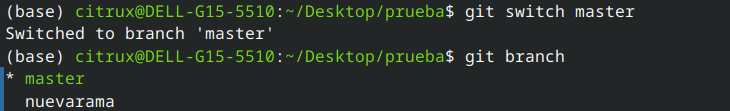
\includegraphics[width=0.9\textwidth]{Imagenes/git_switch.png}
		\end{figure}
		
		Una vez que hemos hecho nuestros cambios en nuestra nueva rama, podemos integrar estos cambios sobre la rama master  (ES NECESARIO CAMBIAR A LA RAMA SOBRE LA QUE SE UNIRÁN LAS RAMAS)
	\end{frame}
	
	\begin{frame}
		\begin{figure}[h]
			\centering
			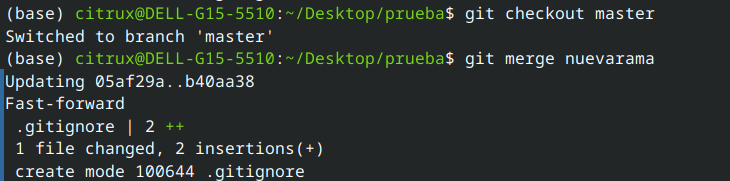
\includegraphics[width=0.9\textwidth]{Imagenes/git_merge.png}
		\end{figure}
		 
		Si ya no necesitamos la rama que hemos creado podemos eliminarla con ``git branch -d nombre\_de\_la\_rama"
		
		\begin{figure}[h]
			\centering
			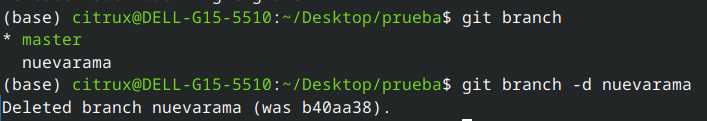
\includegraphics[width=0.9\textwidth]{Imagenes/git_dbranch.png}
		\end{figure}
	
	\end{frame}
	
	\begin{frame}
		\frametitle{¿Pero como comparto mi proyecto?}
		Una opción mas fácil es iniciar el repositorio en algún gestor de repositorios en la nube como \textbf{GitHub} o \textbf{GitLab}, pero nuestro repositorio de ejemplo fue inicializado de manera local, por lo que para subir nuestros cambios a uno de estos gestores, necesitamos iniciar un repositorio vacío sobre ellos. Usamos la instrucción ``git remote add origin url.git" Y luego podremos subir nuestros archivos con ``git push origin master"
		
		\begin{figure}[h]
			\centering
			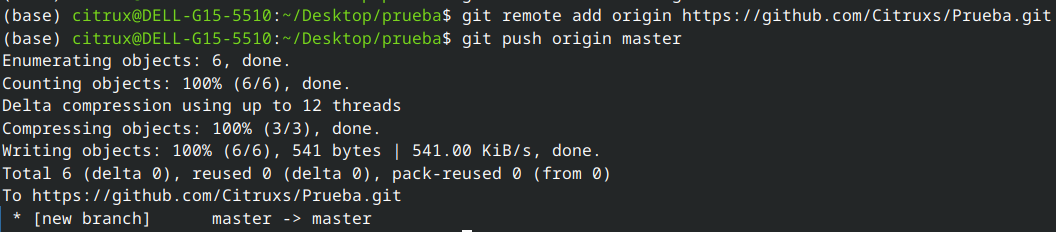
\includegraphics[width=0.9\textwidth]{Imagenes/git_origin.png}
		\end{figure}
	\end{frame}
	
	\begin{frame}
		\frametitle{Uso de GitHub}
		SI ya tenemos algun repositorio en GitHub, podemos clonarlo con ``git clone url.git"
		
		\begin{figure}[h]
			\centering
			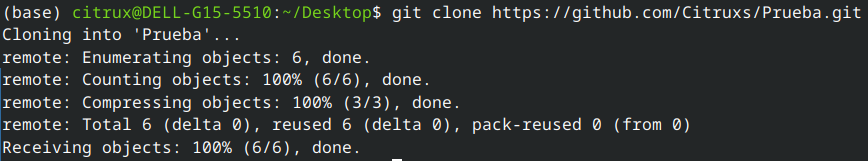
\includegraphics[width=0.9\textwidth]{Imagenes/git_clone.png}
		\end{figure}
		
		Y verificar cambios en el repositorio en la nube con ``git pull origin master"
		
		\begin{figure}[h]
			\centering
			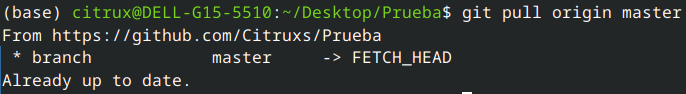
\includegraphics[width=0.9\textwidth]{Imagenes/git_pull.png}
		\end{figure}
		
	\end{frame}
	
	\begin{frame}
	-¿Cómo descargo alguna rama disponible en la nube?\\
	Si tenemos mas de una rama en nuestro repositorio en la nube, podemos cambiarnos a ella, pero lo primero es revisar que ramas tenemos disponibles con: git branch -a
	\begin{figure}[h]
		\centering
		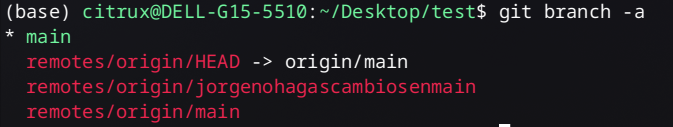
\includegraphics[width=0.9\textwidth]{Imagenes/git_branch_all.png}
	\end{figure}
	
	Una vez que ya hemos visto que ramas tenemos disponibles en nuestro repositorio, podemos cambiarnos a la rama que deseemos con git checkout nombre\_de\_la\_rama
	\end{frame}
	
	\begin{frame}
		\begin{figure}[h]
			\centering
			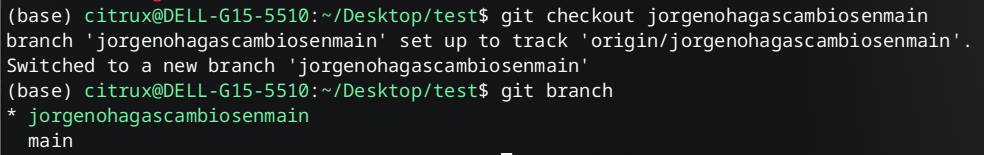
\includegraphics[width=0.9\textwidth]{Imagenes/git_checkout_branch.png}
		\end{figure}
	\end{frame}
	
	\begin{frame}
		\frametitle{Anexo: Claves SSH}
		Si tenemos un repositorio privado o si queremos subir nuestros cambios a un repositorio en la nube, necesitamos configurar nuestra clave SSH.
		
		 Una clave SSH permite que los repositorios en la nube puedan verificar tu identidad sin necesidad de ingresar tu contraseña. Primero tenemos que configurar nuestra clave SSH con: ``ssh-keygen -t rsa", este comando creará nuestras claves SSH pública y privadas en el directorio ``~/.ssh"
	\end{frame}
	
	\begin{frame}
		\begin{figure}[h]
			\centering
			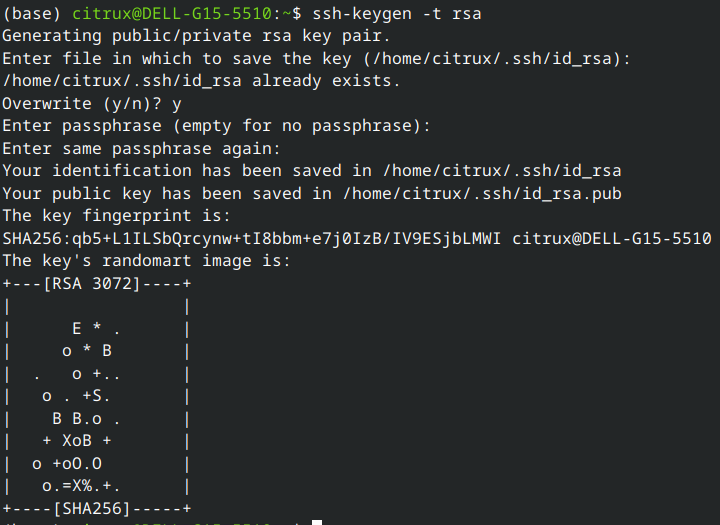
\includegraphics[width=0.9\textwidth]{Imagenes/ssh_keygen.png}
		\end{figure}
	\end{frame}
	
	\begin{frame}
		Una vez generada la clave SSH, podmeos dirigirnos a la carpeta en la que ha sido creada
		
		\begin{figure}[h]
			\centering
			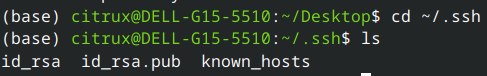
\includegraphics[width=0.9\textwidth]{Imagenes/cd_ssh.png}
		\end{figure}
	
	Y vemos el contenido de la llave publica id\_rsa.pub
	
	\begin{figure}[h]
		\centering
		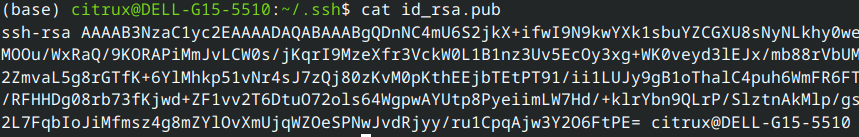
\includegraphics[width=0.9\textwidth]{Imagenes/cat_ssh.png}
	\end{figure}
	
	Copiamos el resultado y nos dirigimos a nuestro gestor de repositorios en la nube como \textbf{GitHub} o \textbf{GitLab}
	\end{frame}
	
	\begin{frame}
		Agregamos la llave SSH en la sección de configuración del administrador de repositorios
		
		\begin{figure}[h]
			\centering
			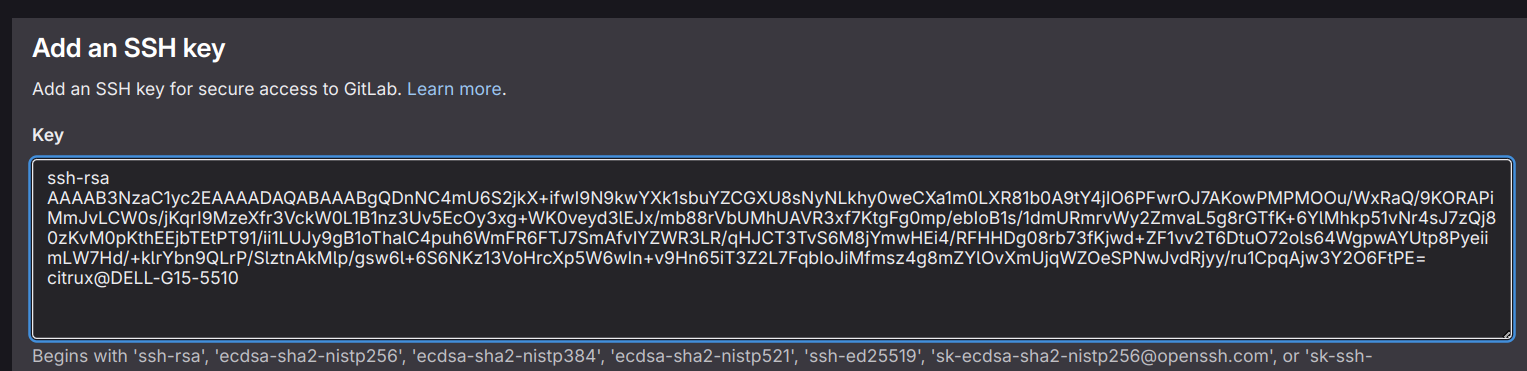
\includegraphics[width=0.9\textwidth]{Imagenes/add_ssh.png}
		\end{figure}
	\end{frame}
	
	\begin{frame}
		\begin{figure}[h]
			\centering
			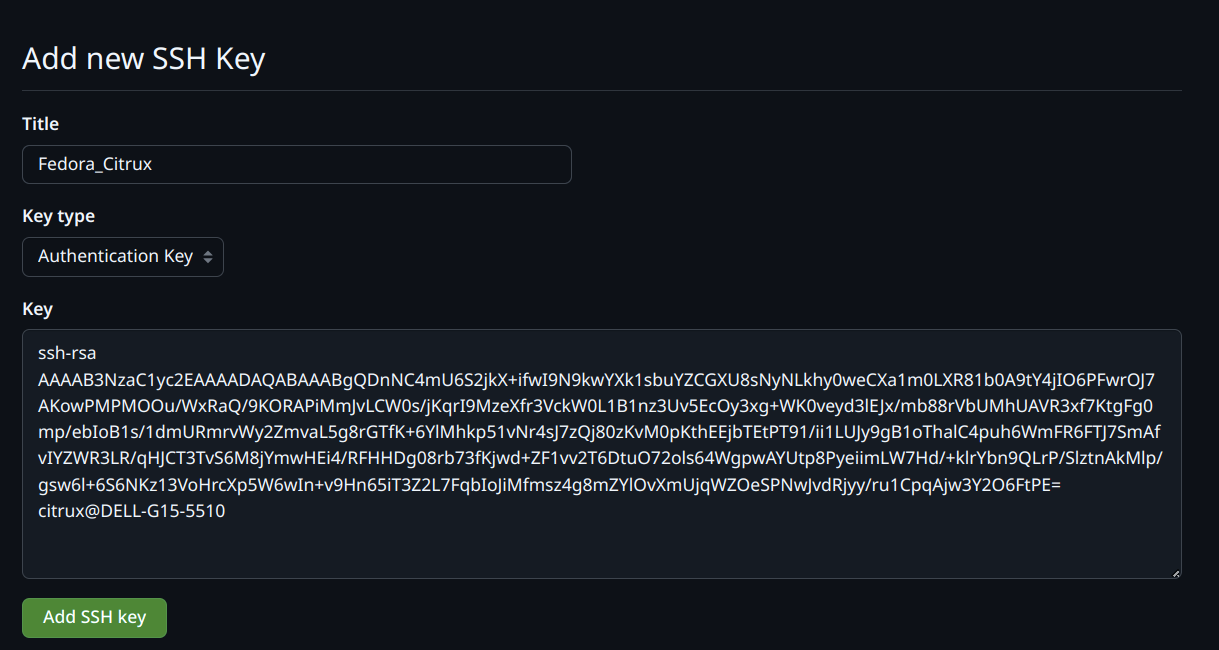
\includegraphics[width=0.9\textwidth]{Imagenes/add_ssh2.png}
		\end{figure}
	\end{frame}
\end{document}